\documentclass[a4paper,11pt,oneside]{book}

\usepackage{color}
\usepackage{graphicx}
\usepackage[utf8]{inputenc}
\usepackage[brazilian]{babel}
\usepackage[hmargin=2cm,vmargin=3.5cm,bmargin=2cm]{geometry}
\usepackage[hidelinks]{hyperref}
\usepackage{amsmath}
\usepackage{amsfonts}
\usepackage{amssymb}


% Global configuration
\setcounter{secnumdepth}{3}		% Add level 3 of sections (can use \subsubsection in books)

% New commands
\newcommand{\todo}[1]{\null \fbox{NOTA: \textcolor{red}{#1}} \\ \null}

\begin{document}

\author{Gustavo Müller Nunes}
\title{Histograma de gradientes para poses de mão em um ambiente automotivo}
\date{June 2014}

\maketitle
\tableofcontents 	% Índice de conteúdos
\listoftables 		% Lista de tabelas
\listoffigures 		% Lista de figuras

%\chapter{Artigos}
%\section{Gesture Components for Natural Interaction with In-Car Devices}
\label{Gesture Components for Natural Interaction with In-Car Devices}

\subsection{Autores}

Martin Zobl, Ralf Nieschulz, Michael Geiger, Manfred Lang, and Gerhard Rigoll

\subsection{Referência}

\hyperref[Gesture Control for use in Automobiles]{Gesture Control for use in Automobiles}

%****************************************************************************************
\section{Gesture Control for use in Automobiles}
\label{Gesture Control for use in Automobiles}

\subsection{Autores}

Suat Akyol, Ulrich Canzler, Klaus Bengler, Wolfgang Hahn

\subsection{Tópicos principais}

\begin{enumerate}
\item Iluminação por LED infravermelho de 950nm
\item Segmentação por "global threshold"
\item Rastreamento de contornos por tamanho, centroide, momentos Hu
\item Medição de velocidade e aceleração
\item Seleção de região por fuzzy
\item filtragem do braço
\item classificador 
\end{enumerate}

%****************************************************************************************
\section{Computer Vision for Interactive Computer Graphics}

No item 3.1 tem uma figura de um mapa de orientação de uma imagem, mas não diz como calcular esse mapa.

Nesse site mostra um exemplo de como calcular o mapa de orientação:
http://answers.opencv.org/question/9493/fingerprint-orientation-map-through-gradient/

Função do MATLAB para plotar os vetores calculadados:
http://www.mathworks.com/help/matlab/ref/quiver.html

Esse artigo talvez seja uma referencia para esse mapa:
http://www.math-info.univ-paris5.fr/~moisan/papers/dequant.pdf

Funções para converter de cartesiano para polar:
http://docs.opencv.org/modules/core/doc/operations_on_arrays.html#polartocart

A idéia então para plotar o mapa de orientação será simplesmente somar nas coordenadas x e y o valor do gradiente normalizado.
Por exemplo, calcular o vetor em cada 10 pixels ou fazer uma media.
\chapter{Introdução}

Reconhecimento de gestos baseado em visão computacional é um assunto bastante pesquisado e já pode ser considerado popular nos dias de hoje, isto porque, a busca por mecanismos que tornem a interação entre homem e máquina mais intuitiva e natural é constante e vem aumentando com o lançamento de plataformas que auxiliam os desenvolvedores nos complexos algoritmos que envolvem essa área.
O lançamento do Kinect, da Microsoft \cite{kinect}, e da plataforma de desenvolvimento da Intel, chamada Intel Perceptual Computing \cite{intel},  ambas com câmeras de profundidade, vem popularizando o desenvolvimento de aplicativos e revolucionando o jeito que interagimos com os jogos e computadores. Em fevereiro de 2013 a Microsoft anunciou que um terço dos consoles Xbox 360 vendidos até o momento tinham o sensor Kinect, totalizando  uma venda de 24 milhões de sensores desde o lançamento do produto em novembro de 2010 \cite{kinect_sales}.

O uso de câmeras em carros e caminhões também tem aumentado nos últimos anos. Sistemas de segurança capazes de verificar se o motorista está saindo indevidamente da faixa, se o veículo está em rota de colisão com algum outro automóvel, pedestre ou objeto e câmeras noturnas, que proporcionam ao motorista uma visão extra quando a  estrada à frente está escura, já são comuns em vários modelos de veículos. Em praticamente todos os modelos da Mercedes Benz, por exemplo, já é possível adquirir sistema de segurança desse tipo. Duas câmeras localizadas atrás do retrovisor e apontadas para a frente do veículo combinadas com um conjunto de radares fazem com que o motorista seja avisado caso haja risco de colisão, entre outras funcionalidades. Dependendo do caso, o veículo pode atuar de forma autônoma e acionar os freios evitando uma colisão ou reduzindo a força do impacto \cite{mercedes_youtube, mercedes_safety}. 

Apesar do uso de câmeras para o lado externo do veículo já ser comum, ainda não é comum o uso dessas câmeras para interação do motorista com a grande quantidade de controles existentes nos carros. Sistemas de navegação, componentes de som e imagem como CD/DVD player, radio, televisão, celulares, computador de bordo, e ar condicionado são alguns exemplos de dispositivos que requererem uma constante interação e demandam uma grande quantidade de botões na região do console. Mesmo que os botões estejam agrupados em diferentes telas em um sistema multimídia, esse tipo de interação ainda exige uma grande atenção do motorista que precisa, na maioria dos casos, localizar visualmente o botão. Nem sempre também o uso dos botões ou da tela é confortável e ergométrico, podendo estar fora do alcance do motorista.

Uma maneira bastante natural de interagir com o veículo é através de comandos de voz e gestos. O sistema de reconhecimento de voz já é bem comum hoje, na maioria dos modelos de carros, mas é facilmente atrapalhado por barulhos internos e externos ao veículo e também interrompe o sistema de áudio, impossibilitando o seu uso caso, por exemplo, o sistema de viva voz estiver ativo. Portanto, um sistema de gestos pode complementar a interface existente, dando mais opção ao usuário na hora de enviar comandos para o veículo.

Nesse sistema gestual de interação do motorista com o veículo, entende-se poses e gestos como sendo movimentos ou poses executados pela mão direta do motorista dentro do campo de visão de uma câmera instalada no teto do carro.
O estudo desse trabalho, portanto, é focado na análise de um sistema capaz de caracterizar as poses de mão para que possam ser classificadas e usadas em um sistema de interface de usuário. Um sistema em tempo real capaz de reconhecer poses de mão e gestos que permita ao motorista interagir com o veículo de forma intuitiva e eficaz. Na figura \ref{fig:visao_aplicacao} tem-se um exemplo de como seria uma pose de mão aberta dentro de um ambiente automotivo.

\begin{figure}[ht!]
	\centering
	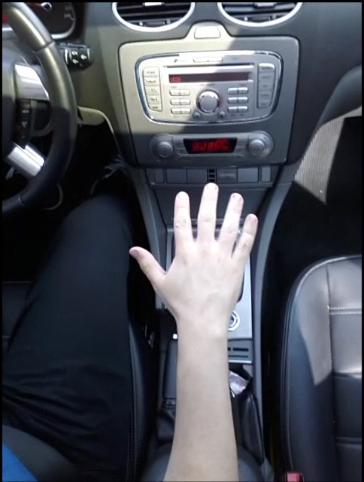
\includegraphics[width=0.3\textwidth]{image/exemplo_visao_aplicacao.png}
	\caption{Exemplo do uso de poses em um ambiente automotivo}
	\label{fig:visao_aplicacao}
\end{figure}

\section{Objetivo}

O objetivo do trabalho é encontrar, em uma imagem obtida no interior do veículo, do ponto de vista do teto e nas mais variadas condições de luminosidade, uma região de interesse com uma alta probabilidade de se ter uma pose de mão. A proposta é estudar o desempenho do histograma de orientações de gradientes (HOG - Histogram of Oriented Gradients) nessas condições e analisar o comportamento das variações dos parâmetros na aplicação e a influência das variáveis do ambiente (mudança de veículo, de motorista e de luminosidade) no algoritmo.
Um balanço entre performance e processamento deve ser levado em consideração, já que o trabalho computacional deve ser reduzido ao máximo para aplicações automotivas.

Um dos primeiros passos no processamento de uma imagem, com o objetivo de se identificar uma pose, é encontrar a região de interesse. Essa região é uma sub imagem onde a mão aparece com mais evidência, eliminando as partes da cena que não são de interesse. Com o escopo reduzido, fica mais robusto aplicar outros algoritmos para a detecção da pose.

A escolha do HOG como descritor para as poses de mão se dá por conta da sua grande robustez contra variações de luminosidade. O HOG foi proposto por \citeonline{dalal2005histograms} que encontraram o melhor conjunto de parâmetros para a representação de seres humanos em diversas situações e poses diferentes. 

O descritor poderia ser usado de duas maneiras diferentes: como um pré classificador para encontrar as regiões mais prováveis de se ter uma mão e assim limitar a imagem em algumas regiões de interesse nas quais um segundo algoritmo seria aplicado. Nesse caso não seria trabalho do HOG dizer qual é a pose, mas sim se é uma mão ou não ou, no máximo, classificar a pose em algum grupo de poses (como feito em \cite{jiang2012robust}). Mas o HOG poderia ser usado também para dizer qual pose é, sem a necessidade de nenhum algoritmo secundário.
Visto que se tem duas aplicações para o HOG, é possível duas configurações diferentes e portanto essas variações devem entrar no escopo desse trabalho.

Trabalha-se, portanto, com a hipótese de que o HOG pode ser parametrizado para encontrar poses de mão. E o conjunto original de parâmetros pode ser modificado para melhor se adequar à aplicação proposta.

\section{Justificativa}

A função principal do motorista deve ser sempre o controle do veículo. Distrações como operar o rádio ou a central multimídia são exemplos constantes de causas de acidentes. Portanto, apenas alguns poucos e curtos momentos podem ser usados para interagir com os comandos do veículo. Em estudos de usabilidade, o controle gestual provou ser mais intuitivo, efetivo \cite{zobl2001usability} e distrair menos do que o uso habitual de botões \cite{geiger2001intermodal}. Por esse motivo, um estudo sobre técnicas para atingir esse objetivo é justificável.

As condições gerais dentro do automóvel incluem uma grande variação de iluminação, mudança de usuário (cor de pele, braço com ou sem vestimentas e vestimentas de cores e estampas diferentes) e fundos não uniformes. Além disso, a aceitação do usuário é um item bastante importante, coisas como uma iluminação artificial visível, restrição de vestimentas e calibração extensiva não podem ser toleradas. Tendo isso em mente, alguns critérios e requisitos para o sistema podem ser estabelecidos:

\begin{itemize}
\item robustez contra ambientes ruidosos
\item iluminação invisível
\item independente de usuário
\item sem calibração ou treinamento pelo usuário
\item pequeno e compreensível conjunto de gestos
\item reação do sistema com o mínimo de latência
\end{itemize}

O estudo de \citeonline{dalal2005histograms} sobre histogramas de orientação de gradientes, aplicado à detecção de humanos variando cada parâmetro do cálculo dos histogramas e encontrando um conjunto de parâmetros que melhor servia para reconhecimento de humanos, virou referência para todos os estudos posteriores na área. Em seu texto ele diz que o uso de histogramas orientados tem muitos precursores \cite{freeman1995orientation, freeman1996computer}, mas que apenas atingiu a maturidade quando combinado com histogramas locais e normalização proposto pela Lowes Scale Invariant Feature Transformation (SIFT) \cite{lowe2004distinctive}. A conclusão a que ele chegou foi que usando histogramas de gradientes locais normalizados, similar ao SIFT, em uma grade com sobreposição se tem ótimos resultados para detecção de humanos, reduzindo falsos positivos em mais de uma ordem de magnitude comparado com Haar wavelets.

\section{Metodologia}

A primeira etapa do projeto é a captura das poses, a pesquisa literária mostra \cite{zobl2004gesture, akyol2000gesture} que o uso de uma câmera infravermelha simples já é adequado para o problema, onde o ambiente é iluminado por infravermelho de curta distância (950nm). A câmera ainda possui um filtro de luz, permitindo apenas que a luz infravermelha seja capturada. Apesar de existir câmeras mais sofisticadas de alta resolução e tecnologias que permitem calcular a distância entre a câmera e o objeto, optou-se por usar a webcam simples por ser mais compatível com os padrões de mercado automotivo. No momento que esse texto foi escrito, as câmeras de profundidade, por exemplo, ainda possuem um preço proibitivo e a quantidade de processamento é bastante limitada em um ambiente embarcado.

As imagens de poses e os vídeos dos gestos serão obtidos em  dois ambientes distintos. Primeiro em um ambiente controlado com fundo homogêneo de cor preta e em uma sala totalmente escura (essa base de dados será usada como referência para os algoritmos implementados). O outro será obtido no interior de um veículo, tanto de dia como de noite. A captura das imagens no interior do veículo é obtida variando tanto o motorista quanto o veículo. Também serão usadas outras bases de dados que não em veículos para comparar a performance do algoritmo nas mais diversas situações.

Próximo passo é a implementação do algoritmo HOG para depois variar os parâmetros e analisar com o melhor conjunto. Pode-se usar como referência a implementação feita pelo MATLAB, que usou os parâmetros de \citeonline{dalal2005histograms} e ainda permite um certo grau de parametrização.

Com relação às poses, vamos analisar a performance de 11 poses diferentes e analisar quais são as poses mais adequadas e que melhor se destacam para o uso em nossa aplicação. Para ter uma noção visual do quanto as poses são diferentes entre si, vamos reduzir as dimensões do vetor de características gerado pelo algoritmo para apenas 3 dimensões. Usando o PCA podemos fazer essa redução e encontrar os 3 auto vetores e auto valores que melhor caracterizam nossas imagens e com isso conseguiremos um gráfico de três dimensões e ter uma perspectiva do quanto os gestos estão agrupados entre si.

\section{Organização da dissertação}

Em construção.


%\chapter{Revisão de Literatura}
%\section{Momentos}

Momentos são medições escalares usadas para caracterizar uma função e capturar suas características mais significativas. São bastante usados a centenas de anos em estatística para descrever a forma de uma função de densidade probabilística e em corpos rígidos para medir a distribuição de massa.
Do ponto de vista matemático, momentos são "projeções" de uma função em uma base polinomial (da mesma forma que, transformada de Fourier é uma projeção em uma base de funções harmônicas).

Definindo então uma imagem como sendo uma função real \( f(x,y) \) de duas variáveis em a compact support \( D \subset \mathbb{R} \subset \mathbb{R} \) e tento uma integral finita diferente de zero. Podemos definir o momento de forma genérica \( M_{pq}^{(f)} \) de uma imagem \( f(x, y) \), onde \( p, q \) são valores não negativos e inteiros e \( r = p + q \) é a ordem do momento, como:

\[ M_{pq}^{(f)} = \iint_D p_{pq} (x, y) f(x, y) \,dx \,dy \]

\section{Momentos invariantes em translação, rotação e escala}

\subsection{Introdução}

Translação, rotação e escala (abreviado como TRS, do inglês \textit{Translation, rotation and scaling}) são as transformações de coordenadas espacial mais simples. TRS é uma transformada de 4 parâmetros, que pode ser descrita como

\[x' = sR \cdot x + t \]

\todo{Verificar link. \\
http://docs.opencv.org/doc/tutorials/imgproc/shapedescriptors/moments/moments.html}
%\chapter{Material e método}

\section{Materiais}
\section{Sistema Proposto}
\section{Discussão}

\subsection{Câmera IR}

\todo{Escrever um pouco sobre as câmeras IR}

\section{Construção da câmera IR}

\todo{Um pouco de texto}

\begin{figure}[ht!]
\centering
\fbox{
  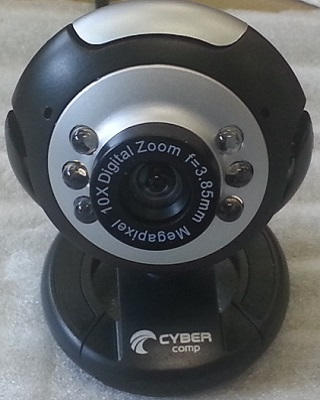
\includegraphics[width=0.3\textwidth]{image/webcam01.jpg}}
  \caption{Webcam sem modificações}
  \label{fig:webcam01}
\end{figure} 

\begin{figure}[ht!]
\centering
\fbox{
  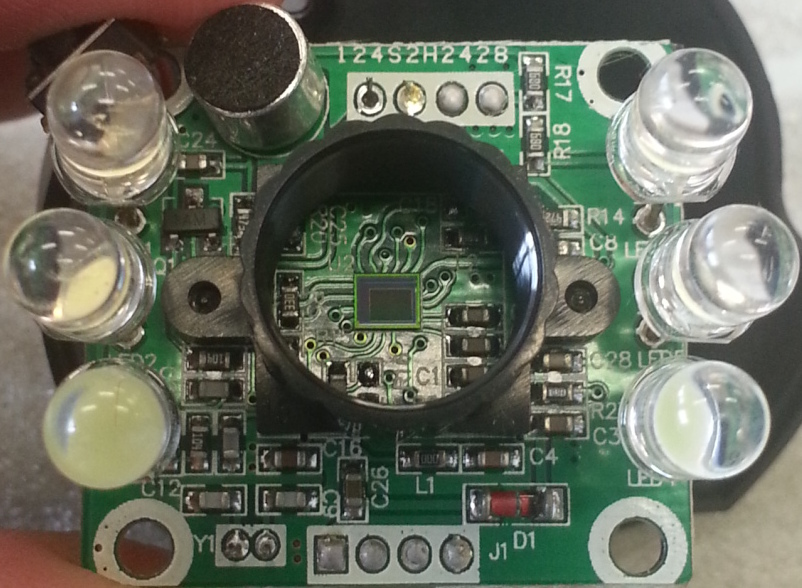
\includegraphics[width=0.3\textwidth]{image/webcam02.jpg}}
  \caption{Webcam sem modificações}
  \label{fig:webcam02}
\end{figure} 

\begin{figure}[ht!]
\centering
\fbox{
  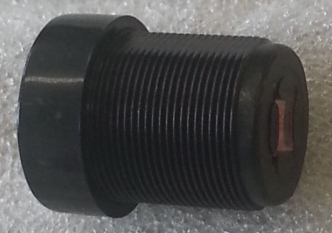
\includegraphics[width=0.3\textwidth]{image/webcam03.jpg}}
  \caption{Webcam sem modificações}
  \label{fig:webcam03}
\end{figure} 

\begin{figure}[ht!]
\centering
\fbox{
  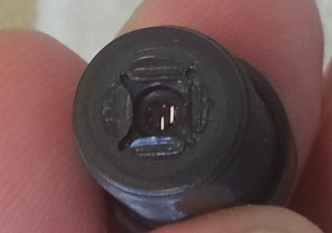
\includegraphics[width=0.3\textwidth]{image/webcam04.jpg}}
  \caption{Webcam sem modificações}
  \label{fig:webcam04}
\end{figure} 

\begin{figure}[ht!]
\centering
\fbox{
  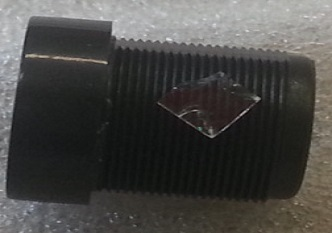
\includegraphics[width=0.3\textwidth]{image/webcam05.jpg}}
  \caption{Webcam sem modificações}
  \label{fig:webcam05}
\end{figure} 

\section{Região de interesse}

Quando o sistema esta inerte e nenhuma mão esta sendo rastreada, podemos criar um região de interesse na imagem para reduzir a área de procura.

%\chapter{Resultados e discussão}
%\chapter{Conclusão}

\begin{thebibliography}{2}

% % % % % % % % % % % % % % % % % % % % % % % % % % % % % % % %
% Gesture Components for Natural Interaction with In-Car devices
% 2001 / Alemanha
\bibitem{ref1} Zobl, M., Nieschulz, R., Geiger, M., Lang M., Rigoll, G.,{Gesture Components for Natural Interaction with In-Car devices}, 2003.

% % % % % % % % % % % % % % % % % % % % % % % % % % % % % % % %
% Gesture control for use in auto-mobiles
% 2000 / Alemanha
\bibitem{ref2} Akyol, S., Canzler, U., Bengler, K., Hahn, W.: Gesture control for use in auto-mobiles. In: Proceedings, MV A 2000 Workshop on Machine Vision Applications, Tokyo, Japan, November 28-30, 2000, IAPR, ISBN 4-901122-00-2 (2000)

% % % % % % % % % % % % % % % % % % % % % % % % % % % % % % % %
% Artigos da Mitsubishi
\bibitem{ref3} W. T. Freeman and M. Roth. Orientation histograms for hand gesture recognition. Intl. Workshop on Automatic Face and Gesture-Recognition, IEEE Computer Society, Zurich, Switzerland, pages 296–301, June 1995.
\bibitem{ref4} W. T. Freeman, K. Tanaka, J. Ohta, and K. Kyuma. Computer vision for computer games. 2nd International Conference on Automatic Face and Gesture Recognition, Killington, VT, USA, pages 100–105, October 1996.

% % % % % % % % % % % % % % % % % % % % % % % % % % % % % % % %
% Real-time Vision-based Infotainment User Determination for Driver Assistance
% 2008 / Estados Unidos
% Artigo com câmera infra no carro e uso de HOG e SVM.
% Criou sua própria base de dados (4 horas diferentes do dia com 8 individuos).
% Possue um descrição do SVM que pode ser usada no futuro.
% [8] Descritor de mão usando Haar-wavelet.
% [9] Detecção de mão usando imagens térmicas.
% [10] Referência ao SIFT. 
\bibitem{ref5} Shinko Y. Cheng and Mohan M. Trivedi. Real-time Vision-based Infotainment User Determination for Driver Assistance, IEEE Intelligent Vehicles Symposium, June 4-6, 2008

% % % % % % % % % % % % % % % % % % % % % % % % % % % % % % % %
% An Effective Crossing Cyclist Detection on a Moving Vehicle 
% 2010 / China
% Tem a formula da normalizacao
% [10] No overlap HOG local features / Mais informação de como calcular o HOG
\bibitem{ref6} An Effective Crossing Cyclist Detection on a Moving Vehicle

\bibitem{ref7} Hand-gesture recognition: comparative study of global, semi-local and local approaches
\bibitem{ref8} Automatic Ship Recognition Robust Against Aspect Angle Changes and Occlusions
\bibitem{ref9} An Extended HOG Model: SCHOG for Human Hand Detection
\bibitem{ref10} A ROBUST METHOD OF FINGERTIP DETECTION IN COMPLEX BACKGROUND
\bibitem{ref11} Deformable HOG-based Shape Descriptor

% % % % % % % % % % % % % % % % % % % % % % % % % % % % % % % %
% Gesture-based control of in-car devices
% Ainda não consegui baixar
\bibitem{ref12} Zobl, M., Geiger, M., Morguet, P., Nieschulz, R., Lang, M.: Gesture-based control of in-car devices. In: VDI-Berichte 1678: USEWARE 2002 Mensch-Maschine-Kommunikation/Design, GMA Fachtagung USEWARE 2002, Darmstadt, Germany, June 11-12, 2002, Dusseldorf, VDI, VDI-Verlag (2002) 305–309

% % % % % % % % % % % % % % % % % % % % % % % % % % % % % % % %
% A usability study on hand gesture controlled operation of in-car devices
% Artigo de justificativa (usabilidade)
\bibitem{ref13} Zobl, M., Geiger, M., Bengler, K., Lang, M.: A usability study on hand gesture controlled operation of in-car devices. In: Abridged Proceedings, HCI 2001 9th Int. Conference on Human Machine Interaction, New Orleans, Louisiana, USA, August 5-10, 2001, New Jersey, Lawrence Erlbaum Ass. (2001) 166–168

% % % % % % % % % % % % % % % % % % % % % % % % % % % % % % % %
% Intermodal differences in distraction effects while controlling automotive user interfaces
% Artigo de justificativa (usabilidade)
\bibitem{ref14} Geiger, M., Zobl, M., Bengler, K., Lang, M.: Intermodal differences in distraction effects while controlling automotive user interfaces. In: Proceedings Vol. 1: Usability Evaluation and Interface Design , HCI 2001 9th Int. Conference on Human Machine Interaction, New Orleans, Louisiana, USA, August 5-10, 2001, New Jersey, Lawrence Erlbaum Ass. (2001) 263–267

% % % % % % % % % % % % % % % % % % % % % % % % % % % % % % % %
% Distinctive Image Features from Scale-Invariant Keypoints
% Descrição do SIFT.
\bibitem{ref15} D. G. Lowe, “Distinctive image features from scale-invariant keypoints,” Int. J. Comput. Vis., vol. 60, no. 2, pp. 91–110, Nov. 2004. 

% % % % % % % % % % % % % % % % % % % % % % % % % % % % % % % %
% Histograms of Oriented Gradients for Human Detection
\bibitem{dalal} Dalal, N. and Triggs, M, "Histograms of Oriented Gradients for Human Detection", in Proc. Of IEEE CVPR2005, vol. 1, pp. 886-893, June 2005.

\bibitem{kinect} http://www.microsoft.com/en-us/kinectforwindows/develop/
\bibitem{intel} http://software.intel.com/en-us/vcsource/tools/perceptual-computing-sdk

\end{thebibliography}

\end{document}